\section{Aprendizado de Maquina}
Se maquinas pensam ou não, o enfoque da IA é executar diretamente um processo que um ser humano aprendeu ao longo dos anos, e não, algo que implicitamente nasceu com ele. Logo, o fluxo mais sistemático para conseguir que uma maquina abstrai-se formalmente um conhecimento seria mapear um estado inicial, aplicar dados para sua aprendizagem e submete-la a outras experiências afim de reafirmar esses conhecimentos. Essa abordagem foi proposta por Turing em 1950, entretanto, o campo de pesquisa conhecido como \textit{\textbf{machine learning}} ou \textbf{aprendizado de maquina} surgiu apenas em 1959 quando o termo nasceu ao ser aplicado em um estudo de redes neurais. Portanto, pode-se brevemente descrever o aprendizado de máquina como métodos computacionais designados a utilizarem de algoritmos precisos de predição juntamente a uma base de conhecimento para aumentar a sua assertividade\cite[1]{turing1950, samuel1959some, mohri2012foundations}.

Nessa sessão será dado um enfoque maior em \textit{machine learning}, primeiramente será introduzido alguns conceitos que serão utilizados a partir dessa sessão. Com os conceitos passados, sera apresentado, de maneira lacônica, a aplicação dos conceitos perante algoritmos de aprendizado de máquina. Por fim, será sugerido algumas ferramentas utilizadas para implementação do \textit{machine learning} e um breve enfoque em como guiaremos esse campo dentro de nossa pesquisa.

\subsection{Conceitos do Aprendizado de Máquina}
Previamente foi dito que, seriam necessários dados de treino, esse dado bruto, como já dito também, contem várias propriedades que podem ser ou não processadas afim de gerar informações, esse dado é conhecido com dados de treinamento e um dado que contém as informações processadas necessárias, inserida por algoritimos ou por fatores externos, é chamado de dado rotulado ou anotado.

As propriedades podem ser utilizadas para classificar um determinado dado, isso as concede o nome de atributo. Também conhecido com \textit{feature} é considerada como um dos fatores mais relevantes para o aprendizado da maquina. O termo conhecido como \textit{feature engineering} ou, em tradução literal, engenharia de atributos, diferente do processo de aprendizagem em si, são baseados diretamente a suas entidades e em como escolher e pré-processar seus atributos chaves afim de otimizar o aprendizado \cite{domingos2012few}.

Esses atributos, dentre outras propriedades, estão em uma massa de dados. Por sua vez serão utilizadas como dado de entrada para um agente. Esse agente tambem pode ser representado, por fins explicativos, como uma simples função \textit{f(x) = y}, o objetivo é treinar o agente para que ele seja capaz de generalizar. Ou seja, capaz de predizer o melhor valor para \textit{y} a partir da entrada \textit{x}. Quando o resultado final depende totalmente do dado de entrada, ou seja, não existem muitas variações que levem a saída a grandes divergências, dizemos que o problema generaliza bem.

Essa função gerada que sucintamente traduz os padrões encontrados entre os dados, gera o que conhecemos como modelo. Muitos deles são utilizados para classificar o dado dentro de um grupo de possibilidades, esse tipo de modelo é descrito como classificador.

Os problemas a serem processados pelos classificadores ou outros modelos possuem um conjunto de  hipóteses. Quando é concebida uma preferencia a uma dessas hipóteses com a premissa de induzir o modelo a tomar uma decisão chamamos esse ato de tendência.

Uma quantidade extensa de hipóteses e dados de entrada não significam uma maquina mais assertiva, quando um agente é treinado para executar mais do que o necessário, um fenômeno peculiar chamado de \textit{overfitting} ou sobre-ajustes acontece, esse evento faz com que a maquina seja capaz de tomar decisões assertivas apenas para um conjunto de dados a qual foi submetida e não consegue predizer novas entradas.

As descrições dadas por Russel \cite[693]{russell2003artificial} ainda se aplicam a conceitos mais complexos que não cabem a essa pesquisa explicitamente. O jeito que é utilizado os dados ou os atributos previamente ditos, podem resultar em diversos tipos de abordagens diferentes.

\subsection{Tipos de Algoritmos}
Os atributos presentes nos dados podem ser utilizados com a premissa de predizer uma determinada hipótese. A aprendizagem supervisionada, como pode-se observar na figura \ref{fig:supervisedlearning}, justifica-se por separar o conjunto de dados em duas bases: teste e treinamento, posteriormente, utilizar as bases para produzir um modelo de predição capaz de satisfazer uma hipótese. Usualmente dentro da aprendizagem supervisionada existe um método que consiste em utilizar de um atributo discreto ou qualitativo e a partir de um indutor gerar o melhor classificador para aquele problema, esse método é chamado classificação. Ainda existe um outro, que se baseia em atributos contínuos, com isso é possível utilizar de predição numérica afim de identificar um modelo dentro do plano cartesiano e prever futuros valores para o mesmo atributo em outras situações, esse método se chama regressão. \cite{hastie2009unsupervised, russell2003artificial}

\begin{figure}[H]
    \centering
    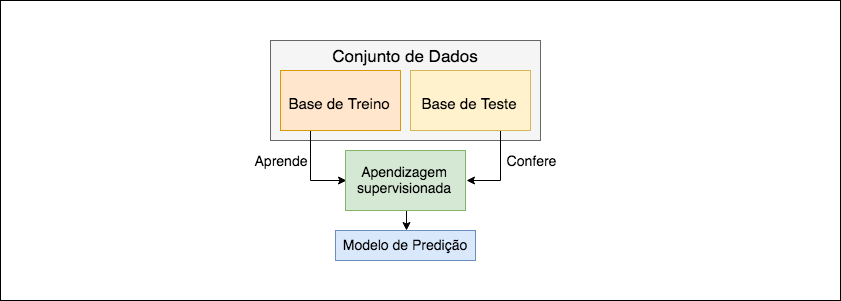
\includegraphics[width=.8\textwidth]{imagens/supervisedlearning.png}
    \caption{Diagrama representando os eventos da aprendizagem supervisionada.}
    \label{fig:supervisedlearning}
\end{figure}

Em contrapartida, existem casos onde os atributos não estarão anotados e a máquina terá que literalmente inferir a probabilidade em toda a base. Esse estilo de aprendizagem se chama aprendizagem não-supervisionada, e o enfoque é utilizar da segregação dos atributos e suas dimensões para inferir resultados. O método mais comum dentro desse estilo é a clusterização que, exemplificado na figura \ref{fig:unsupervised}, se baseia em particionar os dados em grupos dentro de um plano cartesiano tomando de referência um ou mais atributos. Outra pratica utilizada nesse tipo de aprendizagem é redução dimensional, onde resume-se o estado atual de um item para um estado de menor complexidade de dimensões com base nas propriedades chaves \cite{hastie2009unsupervised, mohri2012foundations}.

\begin{figure}[H]
    \centering
    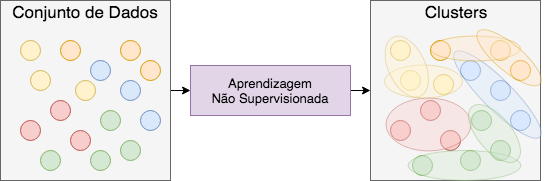
\includegraphics[width=.8\textwidth]{imagens/unsupervised.png}
    \caption{Diagrama representando a clusterização.}
    \label{fig:unsupervised}
\end{figure}

Ainda correlacionado com as últimas explicações, existe um tipo onde é inserido no agente dados anotados e não anotados para predição de todos os itens da base. A aprendizagem semi-supervisionada, suscintamente definida, é a mescla das duas outras aprendizagens. Utiliza da parte anotada (supervisionada) e da lógica de grupos (não-supervisionada), para normalizar e otimizar o resultado final \cite[7]{mohri2012foundations}.

Por último, existem casos onde não teremos dados suficientes para executar outros tipos de aprendizagem, nesse momento a aprendizagem baseada na tradicional tentativa e erro. Nomeada aprendizado por reforço, se observar a figura \ref{fig:reinforcement} pode-se notar que se, consiste em um ambiente (A), responsável por emitir um estado para o componente, feito isso é aplicado uma entrada de dados (e) ao nosso agente (G) que será responsável por tomar a decisão de que ação (a) tomará para a entrada (e) previamente recebida. Essa ação modifica o estado do ambiente e transmite um sinal de reforço visando através do componente (r) para que a aplicação tome a melhor escolha ao longo prazo \cite{kaelbling1996reinforcement, russell2003artificial}.

\begin{figure}[H]
    \centering
    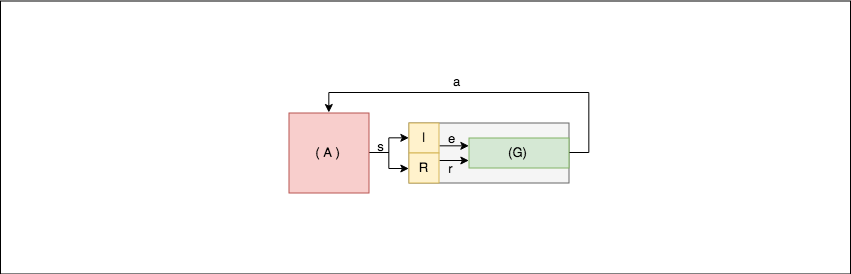
\includegraphics[width=.8\textwidth]{imagens/reinforcement.png}
    \caption{Diagrama apresentando o modelo sequencia ocorrido durante a aprendizagem por reforço.}
    \label{fig:reinforcement}
\end{figure}

Indiferente do tipo ou situação em que o algoritmo se enquadra, a multiplicidade de escolhas propostas pelo \textit{machine learning} gerou várias propostas de aprendizado, algumas até tentando utilizar da estrutura proposta pela neurociência para replicar nossas redes neurais.

\subsection{Algoritimos de Machine Learning}
É essencial entender que existem vários algoritmos de aprendizagem, para todos os tipos já apresentados durante esse referencial. Entretanto, iremos salientar alguns deles.

Um dos algoritimos é o \textit{\textbf{support vector machine}} ou \textbf{SVM}, ele se consiste em construir o máximo de separação entre os pontos, os vetores do SVN possibilitam que, por mais que o algoritmo trabalhe muito bem linearmente, ele crie separações em maiores dimensões. Por ultimo, sua maior vantagem é a flexibilidade, SVN pode suportar funções complexas, porem, é totalmente resistente a \textit{overfitting} \cite[744]{russel2003artificial}.

Diferente de traçar vetores afim de estabelecer funções, existem métodos baseados em sequenciar varias unidades de processamento (similares aos agentes), afim de propagar um input e processa-lo N vezes, por N fórmulas diferentes, afim de encontrar o melhor modelo possível a partir do dado de saída. Basear-se em camadas de unidade de processamento com a proposta de simular o comportamento do cérebro humano ao processar uma informação utilizando camadas de neurônios, essas unidades são fortemente coligadas uma vez que, todas as unidades de todas as camadas são obrigatoriamente interligadas. Essa abordagem ficou conhecida como \textbf{Redes Neurais} ou \textbf{\textit{Neural Network}} \cite{haykin2004comprehensive, russel2003artificial}.

Motivo de retorno dos estudos as Redes Neurais, e também, um dos fatores que podem ser custosos para essa abordagem, o \textbf{\textit{back-propagation}} é o termo utilizado para classificar o ato de ajustar os parâmetros de entrada da sua rede a partir dos dados de saída. Esse ajuste é feito de forma automatizada pela própria massa afim de tentar igualar o valor de saída ao valor esperado. Quando uma rede neural apresenta muitas camadas ela passa a ser considerada uma estrutura de profundida. Infelizmente, o back-propagation não funciona muito bem para redes neurais com muitas camadas. Uma alternativa para isso, seria que nem todos os neurônios fosse interligados, e que os dados tomassem fossem reduzidos por necessidades isoladas se tornando cada vez mais específicos afim de no final propor um conjunto de saidas para parametros esperados, essa abordagem ficou conhecida como \textit{Deep Learning} \cite{lecun2015deep}.

Indiferente da abordagem escolhida, é necessário um conjunto de dados para treinar sua máquina. Portanto, a extração desses dados e posteriormente sua manipulação, exploração e tratamento são essenciais para o sucesso da IA e dos resultados gerados por ela.


